\documentclass[11pt,a4paper]{article}

\usepackage[margin=2.6cm]{geometry}
\usepackage{amsmath,amssymb,amsthm}
\usepackage{booktabs}
\usepackage{graphicx}
\usepackage{microtype}
\usepackage{caption}
\usepackage{algorithm}
\usepackage{algpseudocode}
\usepackage[hidelinks]{hyperref}

\graphicspath{{figures/}}

\theoremstyle{plain}
\newtheorem{proposition}{Proposition}
\theoremstyle{definition}
\newtheorem{remark}{Remark}

\newcommand{\ee}{\mathbf{e}}
\newcommand{\uu}{\mathbf{u}}
\newcommand{\xx}{\mathbf{x}}
\newcommand{\nn}{\mathbf{n}}
\newcommand{\FF}{\mathbf{F}}
\newcommand{\cs}{c_s}

\title{CGLBM: colour-gradient lattice Boltzmann for two-phase flow\\
       \large User reference, derivation, and validation}
\author{Extremumm}
\date{September 2026}

\begin{document}
\maketitle

\begin{abstract}
This document is both the user reference for CGLBM and the record of how its
numerics were derived and validated. Part~\ref{part:using} is what a user needs:
how to build the code, run a case, choose between the two solvers, and read the
output, with a complete reference for every option and configuration field.
Part~\ref{part:method} derives the two models and proves the properties the
implementations rest on. Part~\ref{part:results} reports what they measure.

The short version: CGLBM contains two colour-gradient solvers. The
equation-of-state solver keeps the density ratio independent of the sound-speed
ratio and is quantitative and steady up to a density ratio of about $500$. The
two-population solver ties those two ratios together but reproduces Laplace's
law to $0.3\,\%$ at a density ratio of $10^3$, with spurious currents of
$4.0\times10^{-5}$ --- both better than the reference results of Ba et
al.~\cite{ba2016}. Two ingredients are derived here rather than taken from the
literature: the identity showing that the ``enhanced equilibrium'' of Leclaire
et al.~\cite{leclaire2013} is already contained in the Hermite equilibrium of
the first solver, and an adaptation of the Latva-Kokko recolouring operator
without which the second loses positivity above a density ratio of about four.
\end{abstract}

\tableofcontents

\part{Using CGLBM}
\label{part:using}

\section{What is here}
\label{sec:what}

CGLBM simulates two immiscible fluids with the colour-gradient lattice Boltzmann
method in two dimensions. The library lives under \texttt{src}, the runnable
cases under \texttt{programs}, the Python post-processing in \texttt{PyCGLBM}.

There are two solvers, and choosing between them is the first decision a user
makes.

\begin{center}\small
\begin{tabular}{lll}
\toprule
& \texttt{Solver} (Model A) & \texttt{TwoPopulationSolver} (Model B) \\
\midrule
density ratio comes from & an equation of state & the equilibrium's rest weight \\
sound-speed ratio        & independent of it    & tied to it \\
quantitative to          & $\rho_1/\rho_2 \approx 500$ & $\rho_1/\rho_2 = 10^3$ \\
compressible acoustics   & yes                  & only if $\rho_1/\rho_2$ is small \\
gravity, walls           & yes                  & yes \\
dynamic cases validated  & yes, at ratio 4      & no \\
\bottomrule
\end{tabular}
\end{center}

\noindent
Use \texttt{Solver} unless the density ratio exceeds a few hundred; use
\texttt{TwoPopulationSolver} when it does and the flow is static or slow.
Section~\ref{sec:choosing} gives the reasoning and Part~\ref{part:results} the
measurements.

\section{Building}

Requirements: a C++17 compiler, CMake~$\ge 3.16$, and Python~$\ge 3.9$ for the
post-processing and tests. OpenMP, MPI and CUDA are optional; with any of them
off the corresponding module falls back to one thread, one rank, or the host.

\begin{verbatim}
    cmake --preset gnu          # or --preset clang
    cmake --build --preset gnu
\end{verbatim}

Every program is built twice, \texttt{\_opt} and \texttt{\_dbg}, into
\texttt{bin/} mirroring the \texttt{programs/} tree. Compiler flags live in
\texttt{cmake/CompilerFlags.cmake}; note that \texttt{-ffp-contract=off} is set
deliberately, so that a result is reproducible bit for bit across optimisation
levels.

\section{Running a case}

Each program writes its output to the current directory under fixed names, so
every run needs a directory of its own. \texttt{utilities/run\_case.sh} does
that:

\begin{verbatim}
    utilities/run_case.sh laplace
    pycglbm describe artifacts/laplace
    pycglbm plot artifacts/laplace -o snapshot.png
\end{verbatim}

Every case ships with defaults and accepts overrides on the command line, so
resolution, run length, fluid properties and scheme options are flags rather
than a rebuild:

\begin{verbatim}
    bin/solvers/color_gradient/laplace/laplace_opt --nx=256 --steps=50000
    bin/solvers/color_gradient/laplace/laplace_opt --rho1=100 --sigma=0.05
\end{verbatim}

The run log opens with the full configuration as \texttt{key = value} lines,
which is what the test suite and \texttt{pycglbm} read back rather than
duplicating constants:

\begin{verbatim}
    CaseOutput("artifacts/laplace").parameter("sigma")
\end{verbatim}

\section{Choosing a solver}
\label{sec:choosing}

The two models differ in one structural choice, and everything else follows from
it. \texttt{Solver} carries the density ratio in a two-component equation of
state, so the density and sound-speed ratios are independent --- but the whole
contrast then sits in a single density field, and the pressure reconstructed
from it has to stay smooth across a jump of that size.
\texttt{TwoPopulationSolver} gives each fluid its own rest-particle weight and
hence its own sound speed, which makes the two bulk pressures identically equal
(Proposition~\ref{prop:pressures}) at the cost of tying the sound-speed ratio to
the density ratio: at $\rho_1/\rho_2 = 10^3$ the heavy fluid's sound speed is
$0.022$ in lattice units.

In practice:

\begin{itemize}
\item \textbf{Density ratio below a few hundred, anything dynamic or acoustic:}
      \texttt{Solver}. It is the validated path for the oscillating droplet and
      Rayleigh--Taylor cases.
\item \textbf{Density ratio of $10^3$, static or slow:}
      \texttt{TwoPopulationSolver}, as in \texttt{laplace\_high\_ratio}. Match
      the dynamic viscosities (Section~\ref{sec:viscosity}) --- this matters
      more than any other setting.
\item \textbf{Above $10^3$:} neither is a measurement.
      \texttt{TwoPopulationSolver} runs indefinitely without diverging but does
      not settle; treat it as qualitative.
\end{itemize}

\section{Command-line reference}
\label{sec:cli}

Every solver program accepts the same options. A bare stencil name as the first
argument is also accepted, for compatibility.

\begin{center}\small
\begin{tabular}{lp{9.2cm}}
\toprule
option & meaning \\
\midrule
\multicolumn{2}{l}{\emph{Lattice and run length}}\\
\texttt{-{-}nx=N}, \texttt{-{-}ny=N} & lattice size \\
\texttt{-{-}steps=N}      & number of time steps \\
\texttt{-{-}interval=N}   & write the CSV grids every $N$ steps \\
\texttt{-{-}precision=N}  & significant digits in the CSV output; 6 by default, 17 round-trips \\
\texttt{-{-}threads=N}    & OpenMP threads; implies parallel execution \\
\addlinespace
\multicolumn{2}{l}{\emph{Fluid properties}}\\
\texttt{-{-}rho1=X}, \texttt{-{-}rho2=X} & bulk densities of the two components \\
\texttt{-{-}sigma=X}      & surface tension \\
\texttt{-{-}radius=X}     & prescribed interface radius \\
\texttt{-{-}nu=X}, \texttt{-{-}nu-b=X}   & kinematic shear and bulk viscosity of component~1 \\
\texttt{-{-}nu2=X}, \texttt{-{-}nu-b2=X} & the same for component~2; unset means equal to component~1's. Setting $\nu_2 = \nu_1\rho_1/\rho_2$ matches the dynamic viscosities and makes $\tau$ uniform across the interface \\
\addlinespace
\multicolumn{2}{l}{\emph{Scheme}}\\
\texttt{-{-}stencil=E4|E6|E8} & isotropy order of the colour gradient \\
\texttt{-{-}initial-state=} & \texttt{equilibrium} (default), \texttt{eos} or \texttt{linear}: how $\rho$ and $p$ are laid down at $t=0$ \\
\texttt{-{-}initial-profile=} & \texttt{colour} or \texttt{normalised} (default): which field the initial tanh profile is prescribed in \\
\texttt{-{-}interface-field=} & \texttt{colour} or \texttt{normalised}: which field the colour gradient is taken of \\
\texttt{-{-}surface-tension=} & \texttt{perturbation} or \texttt{csf}: capillary stress in $\Omega^{(2)}$, or a body force from an explicit curvature \\
\texttt{-{-}recolouring=} & \texttt{width} or \texttt{latva-kokko}: segregation from the pressure and a width, or from the density and $\beta$ \\
\texttt{-{-}beta=X}   & segregation strength of \texttt{latva-kokko}, in $(0, 1]$ \\
\texttt{-{-}width=X}, \texttt{-{-}width-init=X} & interface width the recolouring holds, and that of the initial profile \\
\texttt{-{-}help}     & the same list \\
\bottomrule
\end{tabular}
\end{center}

The scheme options apply to \texttt{Solver}. \texttt{TwoPopulationSolver} always
locates the interface with $\varphi_N$, always applies the tension as a body
force, and always recolours with the adapted Latva-Kokko operator of
Proposition~\ref{prop:adapted}; it reads \texttt{-{-}beta} and the fluid
properties, and ignores the rest.

\section{Case configuration reference}
\label{sec:config}

A case is a \texttt{cglbm::lbm::CaseConfig} value handed to a solver. The
scheme itself is in the library and is never repeated per case.

\begin{center}\small
\begin{tabular}{@{}p{5.0cm}p{9.2cm}@{}}
\toprule
field & meaning \\
\midrule
\texttt{name}                & shown in the run log \\
\texttt{nx}, \texttt{ny}     & lattice nodes \\
\texttt{steps}, \texttt{interval} & run length and output frequency \\
\texttt{boundary}            & \texttt{PeriodicY} or \texttt{WallY} (half-way bounce-back); $x$ is always periodic \\
\texttt{initial\_phase}      & a function giving the initial profile at a node; \texttt{droplet\_interface()} and \texttt{cosine\_layer()} are provided \\
\texttt{initial\_profile\_field} & which field that profile is prescribed in \\
\texttt{initial\_state}      & how $\rho$ and $p$ follow from it (Model A only) \\
\texttt{interface\_field},\newline \texttt{surface\_tension},\newline \texttt{recolouring} & scheme options, as above \\
\texttt{stencil}             & isotropy order of the colour gradient \\
\texttt{matched\_pressure\_}\newline\texttt{offset} & set it when the case ties \texttt{p1\_inf} to \texttt{matched\_p1\_inf}, so command-line overrides keep it consistent \\
\texttt{track\_interface}    & append the interface position to \texttt{interface.csv} every step \\
\texttt{parallel}            & run the lattice loops across OpenMP threads \\
\texttt{output\_precision}   & significant digits in the CSV output \\
\addlinespace
\multicolumn{2}{l}{\texttt{physics}, all in lattice units}\\
\texttt{rho1}, \texttt{rho2} & bulk densities \\
\texttt{c1}, \texttt{c2},\newline \texttt{p1\_inf}, \texttt{p2\_inf} & sound speeds and pressures at infinity of the equation of state (Model A) \\
\texttt{alpha2}              & rest-particle weight of component~2 (Model B); $\alpha_1$ follows from the density ratio \\
\texttt{nu}, \texttt{nu\_b},\newline \texttt{nu2}, \texttt{nu\_b2} & kinematic viscosities \\
\texttt{sigma}, \texttt{radius} & surface tension and prescribed interface radius \\
\texttt{gravity}             & uniform acceleration along $-y$; zero switches the body force off entirely \\
\texttt{ch\_width\_init},\newline \texttt{ch\_width\_ope} & interface width at $t=0$ and the one the recolouring holds \\
\texttt{beta}                & Latva-Kokko segregation strength \\
\bottomrule
\end{tabular}
\end{center}

\section{Output and post-processing}

Every program writes four ASCII CSV grids per \texttt{interval} steps, named
after the timestep: \texttt{density}, \texttt{velocity} (with $u_x$ and $u_y$
interleaved), \texttt{phase} and \texttt{pressure}, each suffixed
\texttt{\_<t>.csv}. One row per lattice row, so \texttt{numpy} reads
them as \texttt{array[y, x]}. \texttt{cglbm::lbm::write\_vtk} produces a
ParaView file from the same state.

\begin{verbatim}
    from pycglbm import CaseOutput
    case = CaseOutput("artifacts/laplace")
    case.pressure_jump(30000, inner=5, outer=30)
    case.density_interface_radius(30000)
\end{verbatim}

One point deserves care, because it changes the answer. The phase field's zero
contour is \emph{not} the interface unless the two bulk densities are equal
(Proposition~\ref{prop:interface}). For \texttt{Solver} the interface is the
density midpoint, \texttt{density\_interface\_radius}; for
\texttt{TwoPopulationSolver} the reported phase field is already $\varphi_N$, so
its zero contour is the interface.

\section{Adding a case}

A case is a directory under \texttt{programs} holding one
\texttt{main\_<name>.cpp}. CMake discovers it and builds
\texttt{<name>\_opt}/\texttt{<name>\_dbg} from every source beside it; no CMake
edit is needed. Tests are \texttt{test\_*.py} files placed in a \texttt{tests}
subdirectory, named \texttt{test\_\{marker\}\_\{name\}.py} with markers
\texttt{unit\_test}, \texttt{validation} or \texttt{verification}, plus
\texttt{long} for anything that runs a solver.

\begin{verbatim}
    CaseConfig config;
    config.nx = 128;  config.ny = 128;  config.steps = 10000;
    config.physics.rho1 = 4.;  config.physics.rho2 = 1.;
    config.boundary = Boundary::WallY;
    config.initial_phase = cosine_layer(0.2, /*inverted=*/true);
    Solver(config).run();
\end{verbatim}

\section{Testing}

\begin{verbatim}
    pytest -m unit_test      # fast, no simulation
    pytest --runlong         # includes the tests that run a full case
    ctest --preset gnu       # the same suite through CTest
\end{verbatim}

The unit tests drive the solvers directly on small lattices and check the
invariants each model must hold: mass conservation, the bound on the phase
field, a uniform fluid staying at rest, the equilibrium's moments, and --- for
\texttt{TwoPopulationSolver} --- that neither distribution goes negative.

\section{Pitfalls}
\label{sec:pitfalls}

These are mistakes this project actually made, and they are easy to repeat.

\paragraph{Run long enough to fail.} At high density ratio the viscous
relaxation time grows with the ratio, and a run shorter than one relaxation
time will not diverge no matter how unstable the configuration is. It will
report a plausible number instead. See Section~\ref{sec:runlength}; a density
ratio of $10^3$ in \texttt{Solver} reads $0.96$ at $1.2\times10^4$ steps and is
destroyed at $8.7\times10^4$. Always inspect the time series, not the last
value.

\paragraph{Score against the right radius.} The phase field's zero contour is
not the interface at unequal densities. Scoring Laplace's law against it instead
of the density midpoint changes the answer by tens of per cent.

\paragraph{Match the dynamic viscosities at high contrast.} Equal
\emph{kinematic} viscosity puts $\tau$ at $348$ in the heavy fluid against
$0.85$ in the light one, and the resulting viscous stress absorbs more than half
the capillary force. Set \texttt{-{-}nu2} accordingly.

\paragraph{The interface width is not free.} Widening it resolves a steeper
density profile but makes the curvature vary more across the interface. Both
effects are measurable and they pull in opposite directions.

\part{Method and derivation}
\label{part:method}

\section{Introduction}

A colour-gradient lattice Boltzmann model represents two immiscible fluids by
colouring the particle populations and adding three operators to the collision:
one that generates surface tension, one that segregates the colours, and the
usual relaxation towards equilibrium. The family is attractive because the
surface tension and the interface thickness are set explicitly rather than
emerging from an equation of state, and because it handles large viscosity
ratios well. Its classical weakness is the density ratio.

CGLBM contains two members of the family, and the difference between them is
where the density ratio lives.

\begin{description}
\item[Model A, \texttt{cglbm::lbm::Solver}.] The improved method of Lafarge et
al.~\cite{lafarge2021}. One distribution $f$ for the mixture and one $g$ for the
colour difference, with the density ratio carried by a two-component equation of
state $p = p(\rho,\varphi)$. Density ratio and sound-speed ratio are
independent, so the model is fully compressible.
\item[Model B, \texttt{cglbm::lbm::TwoPopulationSolver}.] The classical model of
Grunau et al.~\cite{grunau1993}, Reis and Phillips, Leclaire et
al.~\cite{leclaire2011,leclaire2012} and Ba et al.~\cite{ba2016}. One
distribution per fluid, with the density ratio carried by a free parameter
$\alpha_k$ in the equilibrium. Density ratio and sound-speed ratio are tied
together.
\end{description}

Sections~\ref{sec:modelA} and~\ref{sec:modelB} set out each model and prove the
properties the implementation relies on. Section~\ref{sec:results} reports what
they measure. Section~\ref{sec:cases} lists the application cases shipped with
the code, and Section~\ref{sec:limits} what is still missing.

Throughout, $\rho_1$ and $\rho_2$ are the bulk densities of the two components,
$\gamma = \rho_1/\rho_2$ the density ratio, and lattice units are used, so
$\delta_x = \delta_t = 1$ and the lattice sound speed is $\cs^2 = 1/3$.

\section{Lattice and notation}

Both models use D2Q9: nine velocities $\ee_i$, weights $w_i$ equal to $4/9$ for
the rest direction, $1/9$ for the four axial ones and $1/36$ for the four
diagonals. The evolution of any population is a collision followed by streaming,
\begin{equation}
  f_i(\xx + \ee_i \delta_t,\, t + \delta_t) = f_i(\xx, t) + \Omega_i(\xx, t),
  \label{eq:lbe}
\end{equation}
and the collision operator is split into three parts,
\begin{equation}
  \Omega_i = \Omega_i^{(1)} + \Omega_i^{(2)} + \Omega_i^{(3)},
  \label{eq:split}
\end{equation}
relaxation towards equilibrium, the surface-tension perturbation, and the
recolouring. What distinguishes the two models is the equilibrium that
$\Omega^{(1)}$ relaxes towards, and what the other two operators act on.

The colour gradient is evaluated with the isotropic stencils of Sbragaglia et
al.\ and Leclaire et al.~\cite{leclaire2011},
\begin{equation}
  \nabla \psi(\xx) \;=\; \sum_\ell W(|\mathbf{c}_\ell|^2)\, \mathbf{c}_\ell\,
  \psi(\xx + \mathbf{c}_\ell),
  \label{eq:isogradient}
\end{equation}
with shell weights chosen so that the lattice tensors match their isotropic
continuum counterparts to fourth (E4), sixth (E6) or eighth (E8) order.
Anisotropy here becomes an anisotropic surface tension, so the order matters;
all results below use E8.

\section{Model A: the equation-of-state model}
\label{sec:modelA}

\subsection{Fields and equilibrium}

Model A carries $f_i$, whose zeroth moment is the mixture density
$\rho = \sum_i f_i$, and $g_i$, whose ratio to $f$ gives the phase field
\begin{equation}
  \varphi = \frac{\sum_i g_i}{\sum_i f_i} \in [-1, 1],
\end{equation}
with $\varphi = +1$ pure component~1 and $\varphi = -1$ pure component~2. The
equilibrium is a Hermite expansion carrying the departure from the ideal gas in
the combination $p - \rho \cs^2$:
\begin{equation}
  f_i^{\mathrm{eq}} = \rho\, w_i \left[ 1 + \frac{\uu\cdot\mathcal{H}^{(1)}_i}{\cs^2}
    + \frac{\uu\uu : \mathcal{H}^{(2)}_i}{2\cs^4} \right]
    + (p - \rho \cs^2)\left[ E_i + w_i \frac{\uu \cdot \mathcal{H}^{(3)}_i}{2\cs^6} \right],
  \label{eq:eqA}
\end{equation}
where $\mathcal{H}^{(n)}_i$ are the Hermite polynomials of $\ee_i$ and $E_i$
collects the second- and fourth-order terms. The pressure comes from the
two-component equation of state, obtained by matching two ideal-gas branches
with their own sound speeds $c_k$ and pressures at infinity $p_{k,\infty}$:
\begin{equation}
  p = \tfrac12\Bigl( \rho \hat{c}^2 - p_{1,\infty} - p_{2,\infty}
    + \sqrt{(p_{2,\infty} - p_{1,\infty} + \rho \bar{c}^2)^2
            + \rho^2 (1-\varphi^2) c_1^2 c_2^2} \Bigr).
  \label{eq:eos}
\end{equation}
This is what decouples the density ratio from the sound-speed ratio, and it is
the reason Model A exists.

\subsection{The enhanced equilibrium is already present}

Leclaire et al.~\cite{leclaire2013} add a third-order term to the
colour-gradient equilibrium to repair its third-order velocity moment, which a
two-component lattice gets wrong whenever the two sound speeds differ. Ba et
al.~\cite{ba2016} restate it as their Eq.~(14) and build their high-density-ratio
model on it. Both name it as the ingredient a model at high density contrast
needs. It is already contained in~\eqref{eq:eqA}, which is not visible by
inspection because \eqref{eq:eqA} never mentions their parameter $\alpha_k$.

\begin{proposition}[Equivalence of the enhanced equilibrium]
\label{prop:enhanced}
Write Ba et al.'s free parameter through
$(\cs^k)^2 = \tfrac{3}{5}(1-\alpha_k)$ and $p_k = \rho_k (\cs^k)^2$. Their term
in excess of the standard equilibrium,
\begin{equation}
  T^{\mathrm{Ba}}_i \;=\; \rho_k w_i \,(3\,\ee_i\!\cdot\!\uu)\;
  \tfrac12\bigl(3(\cs^k)^2 - 1\bigr)\bigl(3|\ee_i|^2 - 4\bigr),
\end{equation}
is identical to the third-order Hermite term of \eqref{eq:eqA},
\begin{equation}
  T^{\mathrm{A}}_i \;=\; (p - \rho\cs^2)\, w_i\,
  \frac{u_x(\mathcal{H}_{yyx} + \mathcal{H}_{xxx}) + u_y(\mathcal{H}_{yyy} + \mathcal{H}_{xxy})}{2\cs^6}.
\end{equation}
\end{proposition}

\begin{proof}
For the third-order Hermite polynomials on D2Q9,
$\mathcal{H}_{xxx} = \xi_x^3 - 3\cs^2 \xi_x$ and
$\mathcal{H}_{yyx} = \xi_y^2\xi_x - \cs^2\xi_x$, so
\begin{equation}
  \mathcal{H}_{xxx} + \mathcal{H}_{yyx}
   = \xi_x\left(\xi_x^2 + \xi_y^2\right) - 4\cs^2 \xi_x
   = \xi_x\left(|\ee_i|^2 - 4\cs^2\right),
\end{equation}
and likewise for $y$. The bracket in $T^{\mathrm{A}}_i$ is therefore
$(\ee_i\!\cdot\!\uu)(|\ee_i|^2 - \tfrac43)$, and since $1/(2\cs^6) = 13.5$,
\begin{equation}
  T^{\mathrm{A}}_i = (p - \rho\cs^2)\, w_i (\ee_i\!\cdot\!\uu)\,
  4.5\left(3|\ee_i|^2 - 4\right).
\end{equation}
On the other side, $\rho_k(\cs^k)^2 = p_k$ gives
$\rho_k\bigl(3(\cs^k)^2 - 1\bigr) = 3\left(p_k - \rho_k \cs^2\right)$, so
\begin{equation}
  T^{\mathrm{Ba}}_i = w_i (\ee_i\!\cdot\!\uu)\,\tfrac32 \cdot 3
  \left(p_k - \rho_k \cs^2\right)\left(3|\ee_i|^2 - 4\right)
  = \left(p_k - \rho_k\cs^2\right) w_i (\ee_i\!\cdot\!\uu)\, 4.5
  \left(3|\ee_i|^2 - 4\right),
\end{equation}
which is $T^{\mathrm{A}}_i$. \qedhere
\end{proof}

The identity is checked numerically over a sweep of sound speed, density and
velocity by \texttt{report\_enhanced\_equilibrium} in
\texttt{programs/unit\_testing/lbm/solver}; the largest disagreement is
$1.1 \times 10^{-14}$. The same correspondence holds for the Chapman--Enskog
source term: Ba et al.'s Eqs.~(17)--(18) correct the energy and diagonal-stress
moments by the divergence of $Q_\alpha = (1.8\alpha_k - 0.8)\rho_k u_\alpha$,
and since $1.8\alpha_k - 0.8 = 1 - 3(\cs^k)^2$ this is
$-3(p_k - \rho_k\cs^2)u_\alpha$, which is precisely the quantity Model A's
source term differentiates, on the same two moments and with the same nine-point
isotropic stencil.

\subsection{Locating the interface}

The interface is where the two components occupy equal volume. Writing $c$ for
the volume fraction of component~1,
\begin{equation}
  c = \frac{\rho\,(1+\varphi)}{2\rho_1},
\end{equation}
the interface is $c = 1/2$. This is \emph{not} $\varphi = 0$.

\begin{proposition}[The phase field is not the interface indicator]
\label{prop:interface}
Let $\varphi_N$ be the bulk-normalised phase field of Ba et al.~\cite{ba2016},
\begin{equation}
  \varphi_N = \frac{\rho_1/\rho_{1,0} - \rho_2/\rho_{2,0}}
                   {\rho_1/\rho_{1,0} + \rho_2/\rho_{2,0}}.
  \label{eq:phin}
\end{equation}
Then $\varphi_N = 2c - 1$; the interface $c = 1/2$ sits at
$\varphi = (\rho_1 - \rho_2)/(\rho_1 + \rho_2)$; and the mixture density takes
the value $\tfrac12(\rho_1 + \rho_2)$ exactly at the interface.
\end{proposition}

\begin{proof}
With partial densities $\rho_1 = c\rho_{1,0}$ and $\rho_2 = (1-c)\rho_{2,0}$,
each scaled term in \eqref{eq:phin} is $c$ and $1-c$, so
$\varphi_N = (c - (1-c))/(c + (1-c)) = 2c - 1$. Setting $\varphi_N = 0$ and
substituting $\varphi = (\rho_1 - \rho_2)/\rho$ gives the stated contour.
Finally $\rho = c\rho_{1,0} + (1-c)\rho_{2,0}$ equals
$\tfrac12(\rho_{1,0}+\rho_{2,0})$ if and only if $c = 1/2$. \qedhere
\end{proof}

At $\gamma = 20$ the half-volume point is $\varphi = 0.905$, and at
$\gamma = 10^3$ it is $\varphi = 0.998$: the zero contour of the colour field
lies deep inside the light fluid, and further inside it the larger the ratio.
Two consequences follow for Model A. Prescribing the initial profile in
$\varphi$ places the droplet nowhere near the prescribed radius --- measured, a
droplet asked for at $R = 10$ is born at $R = 8.41$ at $\gamma = 20$ and at
$R = 6.27$ at $\gamma = 10^3$ --- and the surface-tension operator, which acts
along $\nabla\varphi$, acts in the wrong place. Both are fixed by working with
$\varphi_N$, which is the option \texttt{InterfaceField::BulkNormalised} and the
configuration field \texttt{initial\_profile\_field}.

\begin{remark}
The recolouring operator of Model A needs no change when the interface moves,
because a hyperbolic tangent in $\varphi$ is simultaneously one in $\varphi_N$
of the same width. Writing $\varphi_N = h(\varphi)$ and
$S = \rho_1 + \rho_2$, $D = \rho_2 - \rho_1$, one finds
$h'(\varphi) = 4\rho_1\rho_2/(S + \varphi D)^2$ and
$1 - h(\varphi)^2 = 4\rho_1\rho_2(1-\varphi^2)/(S+\varphi D)^2$, so
$h'(\varphi)\,(1 - \varphi^2) = 1 - \varphi_N^2$ identically: the profile
equation $\nabla\varphi = (1-\varphi^2)\nn/2w$ maps onto
$\nabla\varphi_N = (1-\varphi_N^2)\nn/2w$ with the same $w$.
\end{remark}

\subsection{Applying the surface tension}

Model A's surface tension is a capillary \emph{stress} injected into the
second-order moment, with no curvature ever formed. The operator carries an
explicit $1/\tau$, and the reason is the following.

\begin{proposition}[A post-collision perturbation is amplified by $\tau$]
\label{prop:tau}
Let a perturbation $\Phi_i = O(\varepsilon)$ be added to a BGK collision,
$\Omega_i = -\tfrac{1}{\tau}(f_i - f_i^{\mathrm{eq}}) + \Phi_i$. Then the
momentum flux recovered by the Chapman--Enskog expansion contains the extra
contribution $\tau P^\Phi_{\alpha\beta}$, where
$P^\Phi_{\alpha\beta} = \sum_i \xi_{i\alpha}\xi_{i\beta}\Phi_i$.
\end{proposition}

\begin{proof}
At order $\varepsilon$, $(\partial_{t_1} + \xi\!\cdot\!\nabla) f^{\mathrm{eq}}
= -f^{(1)}/\tau + \Phi^{(1)}$. Substituting this into the second-order Taylor
term of \eqref{eq:lbe} gives, at order $\varepsilon^2$,
\begin{equation}
  \partial_{t_2} f^{\mathrm{eq}}
  + \left(1 - \tfrac{1}{2\tau}\right)(\partial_{t_1} + \xi\!\cdot\!\nabla)f^{(1)}
  + \tfrac12 (\partial_{t_1} + \xi\!\cdot\!\nabla)\Phi^{(1)} = -\tfrac{1}{\tau}f^{(2)}.
\end{equation}
Taking the first moment, the momentum flux picks up
$(1 - \tfrac{1}{2\tau})\Pi^{(1)} + \tfrac12 P^\Phi$. From the order-$\varepsilon$
relation, $\Pi^{(1)} = \Pi^{(1)}_{\mathrm{visc}} + \tau P^\Phi$, so the terms in
$P^\Phi$ total $(\tau - \tfrac12)P^\Phi + \tfrac12 P^\Phi = \tau P^\Phi$. \qedhere
\end{proof}

To inject a capillary stress independent of $\tau$, the operator must therefore
carry $1/\tau$, and Model A's does. The cancellation is exact only where $\tau$
is roughly uniform over the region the operator acts on, and it is not:
\begin{equation}
  \tau = \frac{\rho\nu}{p\,\delta_t} + \frac12
\end{equation}
runs from $5.5$ in the light fluid to $5.0\times10^3$ in the heavy one on the
Laplace case at $\gamma = 10^3$, three lattice nodes apart. Placed on the
interface --- that is, deep on the heavy side --- the operator injects an
amplitude $10^3$ times smaller into populations that stream within a few nodes
into fluid that damps them far faster than they accumulate. Measured, the jump
collapses to $6\,\%$ of $\sigma/R$.

The alternative, taken from Ba et al.~\cite{ba2016}, is to form the curvature
explicitly and apply the tension as a body force,
\begin{equation}
  \FF_s = -\tfrac12 \sigma K \nabla\varphi_N, \qquad
  K = -\nabla\!\cdot\!\nn, \qquad
  \nn = -\frac{\nabla\varphi_N}{|\nabla\varphi_N|},
  \label{eq:csf}
\end{equation}
which reaches the momentum equation through Guo's forcing, whose prefactor
$1 - 1/(2\tau)$ stays in $[\tfrac12, 1]$ however large $\tau$ grows. The factor
$\tfrac12$ makes $|\nabla\varphi_N|/2$ an interface delta function, since
$\varphi_N$ runs from $-1$ to $+1$. This is
\texttt{SurfaceTension::ContinuumSurfaceForce}.

\begin{remark}
An explicit curvature brings a hazard the stress form does not have: $K$ is
built from the \emph{unit} normal and so does not shrink with the gradient it
came from. In the bulk, where that gradient is round-off amplified by
$\mathrm{d}\varphi_N/\mathrm{d}\varphi = \rho_1/\rho_2$, the curvature is a
large random number and the force fails to vanish. Measured at $\gamma = 10^4$,
$|\nabla\varphi_N|$ in the heavy bulk grows from $7\times10^{-12}$ and crosses
$10^{-10}$ by step $9000$. The force is therefore gated at
$|\nabla\varphi_N| > 10^{-6}$, five orders below the physical value of $0.66$.
\end{remark}

\section{Model B: the two-population model}
\label{sec:modelB}

\subsection{Equilibrium and the origin of the density ratio}

Model B carries one distribution per fluid, $f_i^k$ with
$\rho_k = \sum_i f_i^k$ and $\rho = \rho_1 + \rho_2$. Each fluid keeps its own
rest-particle weight:
\begin{equation}
  \phi_i^k = \begin{cases}
    \alpha_k, & i = 0,\\
    (1-\alpha_k)/5, & |\ee_i|^2 = 1,\\
    (1-\alpha_k)/20, & |\ee_i|^2 = 2,
  \end{cases}
  \qquad
  (\cs^k)^2 = \tfrac35 (1 - \alpha_k),
  \label{eq:phik}
\end{equation}
and the equilibrium, with the enhanced first-order term of
Proposition~\ref{prop:enhanced}, is
\begin{equation}
  f_i^{k,\mathrm{eq}} = \rho_k \phi_i^k + \rho_k w_i \left[
    3(\ee_i\!\cdot\!\uu)\Bigl(1 + \tfrac12\bigl(3(\cs^k)^2 - 1\bigr)
      \bigl(3|\ee_i|^2 - 4\bigr)\Bigr)
    + \tfrac92 (\ee_i\!\cdot\!\uu)^2 - \tfrac32 \uu^2 \right].
  \label{eq:eqB}
\end{equation}

\begin{proposition}[Moments of the equilibrium]
\label{prop:momentsB}
The equilibrium \eqref{eq:eqB} satisfies
$\sum_i f_i^{k,\mathrm{eq}} = \rho_k$,
$\sum_i \ee_i f_i^{k,\mathrm{eq}} = \rho_k \uu$ and
$\sum_i \ee_{i\alpha}\ee_{i\beta} f_i^{k,\mathrm{eq}}
 = \rho_k (\cs^k)^2 \delta_{\alpha\beta} + \rho_k u_\alpha u_\beta$.
In particular the enhancement perturbs neither the density nor the momentum.
\end{proposition}

\begin{proof}
$\sum_i \phi_i^k = \alpha_k + 4\frac{1-\alpha_k}{5}
+ 4\frac{1-\alpha_k}{20} = 1$, and the velocity-dependent bracket has zero mean
against $w_i$, giving the zeroth moment. For the first moment write the
enhancement as $3(\ee_i\!\cdot\!\uu)G(|\ee_i|^2)$ with
$G = \tfrac12(3(\cs^k)^2-1)(3|\ee_i|^2 - 4)$, so that $G = -\tfrac12 A$ on the
axial shell and $G = A$ on the diagonal shell, where $A = 3(\cs^k)^2 - 1$. Since
$\sum_{\text{axial}} w_i \xi_\alpha \xi_\beta = \tfrac29 \delta_{\alpha\beta}$
and $\sum_{\text{diag}} w_i \xi_\alpha\xi_\beta = \tfrac19\delta_{\alpha\beta}$,
the enhancement contributes
$3u_\beta\bigl(\tfrac29(-\tfrac12 A) + \tfrac19 A\bigr)\delta_{\alpha\beta} = 0$,
and the plain term gives $\rho_k u_\alpha$. For the second moment,
$\sum_i \phi_i^k \xi_\alpha\xi_\beta = \bigl(\tfrac{2}{5} + \tfrac15\bigr)
(1-\alpha_k)\delta_{\alpha\beta} = \tfrac35(1-\alpha_k)\delta_{\alpha\beta}
= (\cs^k)^2\delta_{\alpha\beta}$, the enhancement is odd in $\ee_i$ and drops
out, and the remaining terms give $\rho_k u_\alpha u_\beta$ as usual. \qedhere
\end{proof}

The density ratio enters through the ``stable interface'' condition of Grunau et
al.~\cite{grunau1993},
\begin{equation}
  \gamma = \frac{\rho_{1,0}}{\rho_{2,0}} = \frac{1 - \alpha_2}{1 - \alpha_1},
  \label{eq:alpharatio}
\end{equation}
which fixes $\alpha_1$ once $\alpha_2$ is chosen. This single relation is what
makes the model work at high contrast.

\begin{proposition}[The bulk pressures are identically equal]
\label{prop:pressures}
With $p = \sum_k \rho_k (\cs^k)^2$ and $\alpha_1$ chosen by
\eqref{eq:alpharatio}, the pressure of pure fluid~1 equals that of pure
fluid~2, for every $\gamma$ and every admissible $\alpha_2$.
\end{proposition}

\begin{proof}
$p_{1} = \rho_{1,0}\,\tfrac35(1-\alpha_1)$ and
$p_{2} = \rho_{2,0}\,\tfrac35(1-\alpha_2)$. By \eqref{eq:alpharatio},
$1 - \alpha_1 = (1-\alpha_2)\rho_{2,0}/\rho_{1,0}$, so
$p_{1} = \rho_{1,0}\tfrac35 (1-\alpha_2)\rho_{2,0}/\rho_{1,0}
= \rho_{2,0}\tfrac35(1-\alpha_2) = p_{2}$. \qedhere
\end{proof}

Proposition~\ref{prop:pressures} is the whole advantage of Model B. The pressure
is continuous across the interface however large the density ratio, and each
$\rho_k$ has its own smooth profile, so nothing has to resolve a jump of
$\gamma$ within a single field. The price is that \eqref{eq:alpharatio} ties the
sound speeds to the density ratio: at $\gamma = 10^3$ with $\alpha_2 = 0.2$ the
heavy fluid's sound speed is $\cs^1 = 0.022$ in lattice units.

\subsection{The recolouring must be adapted to the density ratio}
\label{sec:recolour}

Latva-Kokko and Rothman's segregation operator, as Ba et al.\ write it, splits
the post-perturbation total $f_i^\dagger$ by mass fraction and pushes colour
along the colour gradient in proportion to the \emph{lattice} weight:
\begin{equation}
  f_i^{1\ddagger} = \frac{\rho_1}{\rho} f_i^\dagger
   + \beta\, w_i\, \frac{\rho_1\rho_2}{\rho}\cos\phi_i, \qquad
  \cos\phi_i = \frac{\ee_i\!\cdot\!\nabla\varphi_N}{|\ee_i|\,|\nabla\varphi_N|},
  \label{eq:lk}
\end{equation}
and correspondingly for fluid~2 with the opposite sign. This is correct when the
two fluids share a rest weight, and fails otherwise.

\begin{proposition}[Latva-Kokko loses positivity at modest density ratio]
\label{prop:lkfails}
Consider a node at which the two fluids occupy equal volume, so
$\rho_1 = \gamma/2$ and $\rho_2 = 1/2$ with $\rho_{2,0} = 1$, and take an axial
direction. Under \eqref{eq:lk}, $f_i^{2\ddagger} < 0$ whenever
\begin{equation}
  \gamma \;>\; \frac{2(1-\alpha_2)}{5\,\beta\,w_i},
  \label{eq:lkthreshold}
\end{equation}
which for $\alpha_2 = 0.2$, $\beta = 0.7$ and $w_i = 1/9$ is
$\gamma > 4.11$.
\end{proposition}

\begin{proof}
By \eqref{eq:phik} and \eqref{eq:alpharatio}, the axial populations are
$f_i^1 = \rho_1 (1-\alpha_1)/5 = \tfrac{\gamma}{2}\cdot\tfrac{1-\alpha_2}{5\gamma}
= (1-\alpha_2)/10$ and
$f_i^2 = \rho_2 (1-\alpha_2)/5 = (1-\alpha_2)/10$; note both are independent of
$\gamma$. Hence $f_i^\dagger = (1-\alpha_2)/5$ and fluid~2's share of it is
$(\rho_2/\rho) f_i^\dagger$. The push is $\beta w_i \rho_1\rho_2/\rho$, so
\begin{equation}
  \frac{\text{push}}{\text{share}}
  = \frac{\beta w_i \rho_1 \rho_2/\rho}{(\rho_2/\rho) f_i^\dagger}
  = \frac{\beta w_i \rho_1}{f_i^\dagger}
  = \frac{\beta w_i \gamma/2}{(1-\alpha_2)/5}
  = \frac{5\beta w_i \gamma}{2(1-\alpha_2)},
\end{equation}
and $f_i^{2\ddagger} < 0$ once this exceeds one. \qedhere
\end{proof}

At $\gamma = 10^3$ the ratio is $243$: the light fluid's distribution is driven
negative by more than two orders of magnitude, and the run is destroyed within
ten steps. Measured, Model B with \eqref{eq:lk} is accurate at $\gamma = 2$,
gives $-69\,\%$ at $\gamma = 5$ and produces \texttt{nan} from $\gamma = 30$
upwards --- which brackets the threshold of Proposition~\ref{prop:lkfails}
closely. Figure~\ref{fig:recolouring} plots the criterion.

Leclaire et al.~\cite{leclaire2012} report adapting the operator ``for the case
of variable density ratios'', and Leclaire et al.~\cite{leclaire2011} credit
that adaptation with reaching $\gamma \sim 10^4$. Their formulation was not
available to this work, so the following form is derived from the two
requirements the operator has to meet rather than transcribed.

\begin{proposition}[An adapted segregation operator]
\label{prop:adapted}
Replace $w_i$ in \eqref{eq:lk} by the mixture's own rest weight,
\begin{equation}
  \Phi_i \;=\; \frac{\rho_1 \phi_i^1 + \rho_2 \phi_i^2}{\rho}
  \;=\; \frac{f_i^{\mathrm{eq}}(\rho, \mathbf{0})}{\rho}.
  \label{eq:adapted}
\end{equation}
Then \emph{(i)} each fluid's mass is conserved exactly; \emph{(ii)} near
equilibrium both distributions remain non-negative for every $\beta \le 1$ and
every density ratio; and \emph{(iii)} the operator reduces to \eqref{eq:lk} when
$\alpha_1 = \alpha_2$.
\end{proposition}

\begin{proof}
\emph{(i)} $\Phi_i$ depends on $i$ only through $|\ee_i|^2$, and
$\cos\phi_i$ is odd under $\ee_i \mapsto -\ee_i$, so
$\sum_i \Phi_i \cos\phi_i = 0$ shell by shell; the split by mass fraction
already conserves $\rho_1$ and $\rho_2$, so the push adds nothing.
\emph{(ii)} Near equilibrium $f_i^\dagger \simeq \rho_1\phi_i^1 + \rho_2\phi_i^2
= \rho\,\Phi_i$. The ratio of the push to fluid~2's share is then
\begin{equation}
  \frac{\beta \Phi_i \rho_1\rho_2/\rho}{(\rho_2/\rho)\,\rho\,\Phi_i}
  = \beta\frac{\rho_1}{\rho} \le \beta \le 1,
\end{equation}
since $\rho_1 \le \rho$; the same bound with $\rho_2$ in place of $\rho_1$
covers fluid~1. \emph{(iii)} If $\alpha_1 = \alpha_2 = \alpha$ then
$\phi_i^1 = \phi_i^2 = \phi_i$ and $\Phi_i = \phi_i$, which is $w_i$ for the
standard weights. \qedhere
\end{proof}

The bound in part \emph{(ii)} is uniform in $\gamma$, which is the property
\eqref{eq:lk} lacks. Measured over fifty steps of a droplet, the minimum of
$f_i^k$ over the whole lattice is exactly zero at $\gamma = 20$, $10^3$ and
$10^5$, and $|\varphi_N|$ is exactly $1$: the phase field is bounded because the
populations are, not because anything clamps it.

\subsection{The relaxation time must be matched, not the kinematic viscosity}
\label{sec:viscosity}

By Proposition~\ref{prop:pressures} the two bulk pressures are equal, so with
$\tau = \mu/(p\,\delta_t) + \tfrac12$ giving both fluids the same
\emph{kinematic} viscosity --- Ba et al.'s choice, $\nu = 0.1667$ --- puts
$\tau = 348$ in the heavy fluid against $0.85$ in the light one. A BGK collision
at $\tau = 348$ leaves a viscous stress large enough to absorb most of the
capillary force. Measured on a relaxed droplet at $\gamma = 10^3$: integrating
the solver's own capillary force along the outward normal gives $0.00413$,
within $3\,\%$ of $\sigma/R$, while the pressure jump is $0.00176$ --- $43\,\%$
of the force actually applied. The tension then reads $63\,\%$ low.

Ba et al.\ carry this with a multiple-relaxation-time collision, which relaxes
the ghost moments at their own rate. The alternative used here is to match the
\emph{dynamic} viscosities, which makes $\tau$ uniform at $0.85$ and needs no
MRT. It is a different physical case --- a viscosity ratio of $\gamma$ rather
than of one --- and the shipped case states so.

\section{Algorithms}

\begin{algorithm}[htbp]
\caption{One step of Model A, \texttt{cglbm::lbm::Solver}}
\label{alg:A}
\begin{algorithmic}[1]
\State $S_i \gets S_F + S_{Sp} + S_t$ \Comment{Guo forcing, third-moment and temporal corrections}
\State $\Omega^{(1)}_i \gets$ regularised relaxation of $f - f^{\mathrm{eq}} + S/2$ at $\tau_\nu, \tau_b$
\If{tension is a stress}
  \State $\Omega^{(2)}_i \gets \sigma w_i \bigl(\ldots\bigr)/(4|\nabla\varphi_N|\cs^4)$, divided by $\tau_\nu, \tau_b$
\EndIf
\State $\Omega^{(3)}_i \gets w_i\, p\,(1-\varphi^2)(\ee_i\!\cdot\!\nn) / (2 W \cs^2)$ \Comment{recolouring}
\State $f_i(\xx + \ee_i) \gets f^{\mathrm{eq}}_i + \Omega^{(1)}_i + \Omega^{(2)}_i + S_i/2$
\State $g_i(\xx + \ee_i) \gets f_i(\xx+\ee_i)\,\varphi(\xx) + \Omega^{(3)}_i$
\State $\rho \gets \sum_i f_i$; \quad $\uu \gets (\sum_i \ee_i f_i + \FF\delta_t/2)/\rho$
\State $\varphi \gets \sum_i g_i / \sum_i f_i$; \quad $p \gets p(\rho, \varphi)$ by \eqref{eq:eos}
\State $\varphi_N \gets$ \eqref{eq:phin}; \quad $\nabla\varphi_N \gets$ \eqref{eq:isogradient}
\If{tension is a body force}
  \State $\nn \gets -\nabla\varphi_N/|\nabla\varphi_N|$; \quad $K \gets -\nabla\!\cdot\!\nn$;
         \quad $\FF_s \gets -\tfrac12\sigma K \nabla\varphi_N$
\EndIf
\State $f^{\mathrm{eq}}_i \gets$ \eqref{eq:eqA}
\end{algorithmic}
\end{algorithm}

\begin{algorithm}[htbp]
\caption{One step of Model B, \texttt{cglbm::lbm::TwoPopulationSolver}}
\label{alg:B}
\begin{algorithmic}[1]
\State $\rho_k \gets \sum_i f_i^k$; \quad $\rho \gets \rho_1 + \rho_2$;
       \quad $p \gets \sum_k \rho_k (\cs^k)^2$
\State $\varphi_N \gets (\rho_1/\rho_{1,0} - \rho_2/\rho_{2,0}) / (\rho_1/\rho_{1,0} + \rho_2/\rho_{2,0})$
\State $\nabla\varphi_N \gets$ \eqref{eq:isogradient}; \quad
       $\nn \gets -\nabla\varphi_N/|\nabla\varphi_N|$
\State $K \gets n_x n_y(\partial_y n_x + \partial_x n_y) - n_x^2 \partial_y n_y - n_y^2 \partial_x n_x$
\State $\FF \gets -\tfrac12 \sigma K \nabla\varphi_N + \FF_{\mathrm{gravity}}$
\State $\uu \gets \bigl(\sum_k\sum_i \ee_i f_i^k + \FF \delta_t/2\bigr)/\rho$
\State $\mu \gets c\,\mu_1 + (1-c)\,\mu_2$ with $c = (1+\varphi_N)/2$;
       \quad $\tau \gets \mu/(p\delta_t) + \tfrac12$
\ForAll{$k \in \{1,2\}$}
  \State $f_i^k \gets f_i^k - \tfrac{1}{\tau}(f_i^k - f_i^{k,\mathrm{eq}})
         + \bigl(1 - \tfrac{1}{2\tau}\bigr)\tfrac{\rho_k}{\rho} S_i \delta_t$
         \Comment{$f^{k,\mathrm{eq}}$ by \eqref{eq:eqB}}
\EndFor
\State $f_i^\dagger \gets f_i^1 + f_i^2$
\State $f_i^{1} \gets \tfrac{\rho_1}{\rho}f_i^\dagger
       + \beta \Phi_i \tfrac{\rho_1\rho_2}{\rho}\cos\phi_i$;
       \quad $f_i^{2} \gets f_i^\dagger - f_i^{1}$ \Comment{$\Phi_i$ by \eqref{eq:adapted}}
\State $f_i^k(\xx + \ee_i) \gets f_i^k(\xx)$
\end{algorithmic}
\end{algorithm}

\part{Validation}
\label{part:results}

\section{Results}
\label{sec:results}

\subsection{Laplace's law against the density ratio}

Figure~\ref{fig:sweep} is the summary result. A static droplet is relaxed and
the pressure jump measured against the radius at which the interface actually
settles; for Model A that is the density midpoint, which by
Proposition~\ref{prop:interface} is the physical interface, and for Model B it
is the $\varphi_N = 0$ contour, which is the same surface.

Three things are worth reading off it. Model A in its original configuration is
about $10\,\%$ low and stays there --- $0.894$ at $\gamma = 10$, $0.904$ at
$100$, $0.898$ at $200$ --- so the error is a property of the scheme rather than
of the density ratio, until $\gamma = 500$ where it collapses to $0.618$. With
the interface located by $\varphi_N$ and the tension applied as a body force it
reads $1.021$ and is flat to a tenth of a per cent from $\gamma = 5$ to $200$;
its spurious currents also \emph{fall} with the density ratio, from
$2.2\times10^{-5}$ to $7.5\times10^{-6}$, which is the opposite of what the
other two do. And Model B is within $0.3\,\%$ over three decades, from $1.0026$
at $\gamma = 2$ to $1.0030$ at $10^3$, with spurious currents rising gently from
$8.4\times10^{-6}$ to $4.0\times10^{-5}$.

\begin{figure}[htbp]
  \centering
  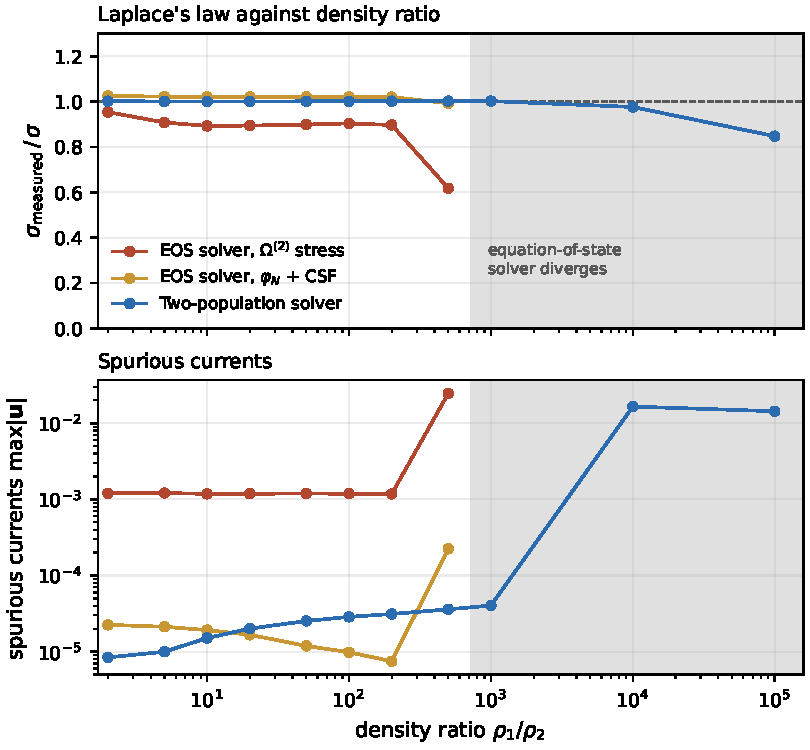
\includegraphics[width=0.78\textwidth]{fig_sweep.pdf}
  \caption{Measured interfacial tension and spurious currents against the
  density ratio, all from runs of $1.2\times10^5$ steps (Model A) or
  $6\times10^4$ (Model B). Model A's original configuration sits about $10\,\%$
  low and holds there to $\gamma = 200$; with the interface located by
  $\varphi_N$ and the tension applied as a body force it reads $1.021$, flat to
  a tenth of a per cent from $\gamma = 5$ to $200$, and its spurious currents
  \emph{fall} with the density ratio. Both diverge at $10^3$. Model B is within
  $0.3\,\%$ across three decades.}
  \label{fig:sweep}
\end{figure}

\subsection{How long a run has to be}
\label{sec:runlength}

The most important methodological point in this report is negative. At the
viscosity the Laplace case ships with, the viscous relaxation time
$\tau = \rho\nu/(p\delta_t) + \tfrac12$ grows with the density ratio, and a run
of $3\times10^4$ steps covers

\begin{center}
\begin{tabular}{lrr}
\toprule
density ratio & $\tau$ in the heavy fluid & relaxation times in $3\times10^4$ steps \\
\midrule
$20$    & $1.0\times10^2$ & $299$ \\
$10^3$  & $5.0\times10^3$ & $6.0$ \\
$10^4$  & $5.0\times10^4$ & $0.60$ \\
$10^5$  & $5.0\times10^5$ & $0.06$ \\
\bottomrule
\end{tabular}
\end{center}

An unstable configuration run for less than one relaxation time does not
diverge; it simply has not got there yet. Figure~\ref{fig:history} shows what
this looks like at $\gamma = 10^3$. Model A with the tension applied as a body
force reads a plausible $0.963$ at $1.6\times10^4$ steps, $0.936$ at
$2.8\times10^4$, $0.868$ at $4.0\times10^4$ and $0.845$ at $5.2\times10^4$; by
$6.4\times10^4$ the pressure jump has inverted sign, and the run is gone by
$7.2\times10^4$. Its stress-based configuration goes the same way sooner.
Earlier versions of this project reported a density ratio of $10^3$, and before
that $10^5$, on exactly such trajectories. Every figure in this report is taken
from runs of at least $1.2\times10^5$ steps with the whole time series
inspected, and the same discipline is worth applying to any new case.

\begin{figure}[htbp]
  \centering
  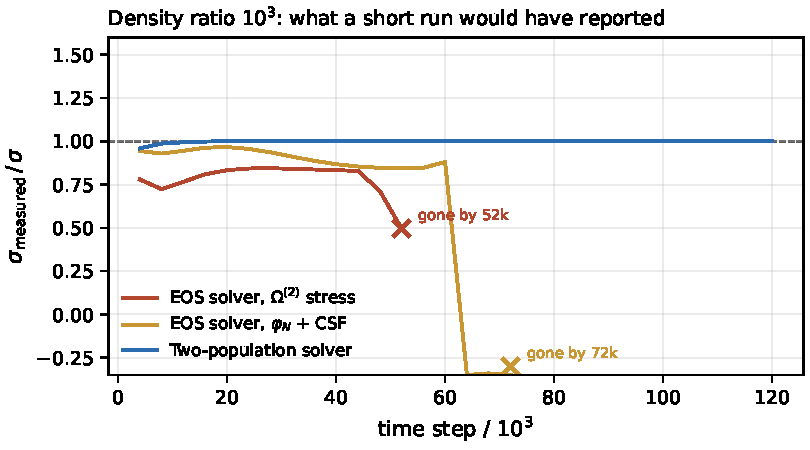
\includegraphics[width=0.78\textwidth]{fig_history.pdf}
  \caption{The measured tension against time at $\gamma = 10^3$. Both
  configurations of Model A look healthy for tens of thousands of steps before
  collapsing. Model B is flat.}
  \label{fig:history}
\end{figure}

\subsection{Interface structure}

Figure~\ref{fig:profiles} shows why. The two models settle on nearly the same
density profile, so the difference is not in how they resolve the interface. It
is in the pressure: Model A reconstructs it from a single density field through
\eqref{eq:eos} and carries a $13\,\%$ interfacial excursion, while in Model B
the two bulk pressures are equal by Proposition~\ref{prop:pressures} and the
profile is flat. The same figure shows Proposition~\ref{prop:interface} in
practice --- Model A's colour field crosses zero about four lattice nodes
outside the interface, which is why scoring Laplace's law against that contour
gives the wrong answer.

\begin{figure}[htbp]
  \centering
  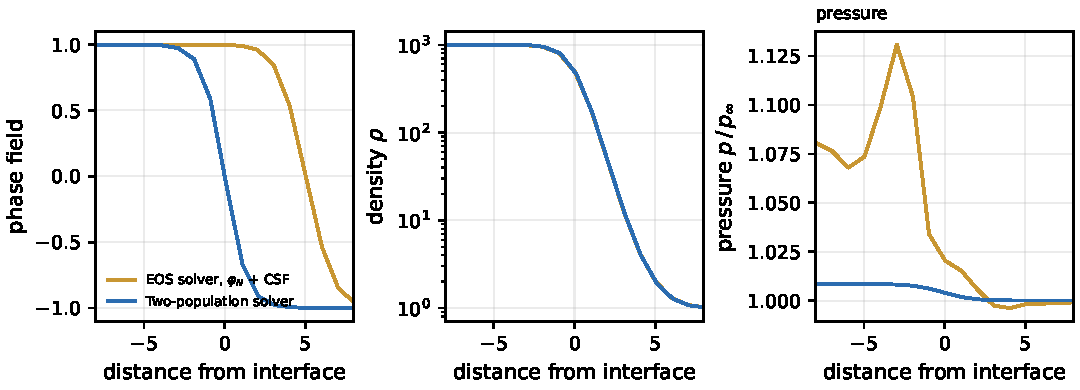
\includegraphics[width=\textwidth]{fig_profiles.pdf}
  \caption{Phase field, density and pressure across the interface at
  $\gamma = 10^3$, each centred on the density midpoint --- the physical
  interface in both models by Proposition~\ref{prop:interface}. The two models
  produce essentially the \emph{same} density profile, and differ in the other
  two panels. Model A's phase field is the colour field, whose zero contour sits
  some four nodes outside the interface, while Model B reports $\varphi_N$,
  which crosses zero on it. And Model A's pressure, reconstructed from a single
  density field through \eqref{eq:eos}, carries a $13\,\%$ excursion where
  Model B's is flat to a fraction of a per cent.}
  \label{fig:profiles}
\end{figure}

\subsection{Spurious currents}

Figure~\ref{fig:currents} shows the residual velocity field of Model B at
$\gamma = 10^3$. The characteristic eight-lobe pattern of a colour-gradient
model is present but small.

\begin{figure}[htbp]
  \centering
  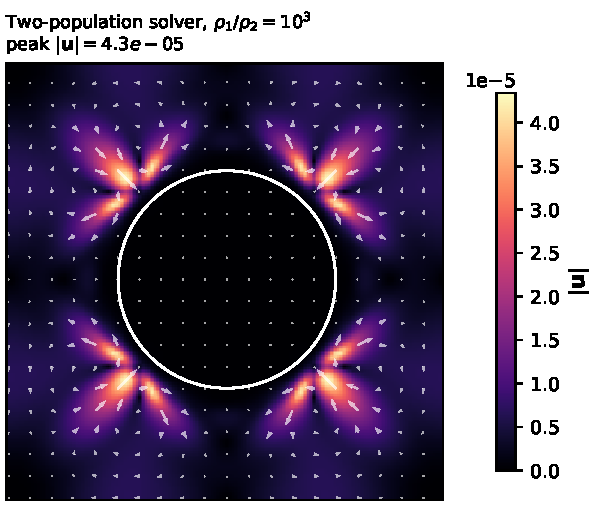
\includegraphics[width=0.62\textwidth]{fig_currents.pdf}
  \caption{Spurious currents around the relaxed droplet, Model B at
  $\gamma = 10^3$. The white contour is $\varphi_N = 0$.}
  \label{fig:currents}
\end{figure}

\subsection{The recolouring criterion}

Figure~\ref{fig:recolouring} plots Proposition~\ref{prop:lkfails} against
Proposition~\ref{prop:adapted}: the colour the operator moves, divided by the
colour available to move. The original form crosses one at
$\gamma \approx 4.1$; the adapted form is bounded by $\beta$ at every ratio.

\begin{figure}[htbp]
  \centering
  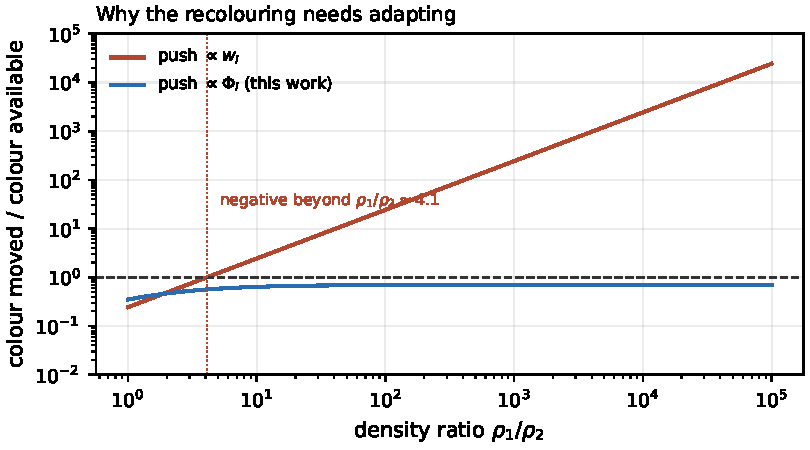
\includegraphics[width=0.78\textwidth]{fig_recolouring.pdf}
  \caption{Why the segregation operator has to be adapted. Above the dashed
  line a distribution is driven negative.}
  \label{fig:recolouring}
\end{figure}

\subsection{Comparison with the literature}

\begin{center}
\begin{tabular}{lrrrr}
\toprule
& \multicolumn{2}{c}{this work, Model B} & \multicolumn{2}{c}{Ba et al.~\cite{ba2016}} \\
\cmidrule(lr){2-3}\cmidrule(lr){4-5}
density ratio & $\sigma_{\mathrm{meas}}/\sigma$ & $\max|\uu|$
              & $\sigma_{\mathrm{meas}}/\sigma$ & $\max|\uu|$ \\
\midrule
$100$   & $1.0023$ & $2.9\times10^{-5}$ & $1.0069$ & $6.8\times10^{-5}$ \\
$10^3$  & $1.0030$ & $4.0\times10^{-5}$ & $1.0074$ & $1.25\times10^{-4}$ \\
\bottomrule
\end{tabular}
\end{center}

The cases are the same: $R = 25$ in $100^2$, $\sigma = 0.1$, $\alpha_2 = 0.2$,
$\beta = 0.7$, periodic on both axes. The difference in configuration is the
viscosity, as set out in Section~\ref{sec:viscosity}. Both quantities here are
better than the reference, and the runs are converged --- the last six reports
of each agree to every digit printed.

\section{Application cases}
\label{sec:cases}

\begin{center}\small
\begin{tabular}{llrrl}
\toprule
program & model & lattice & $\rho_1/\rho_2$ & purpose \\
\midrule
\texttt{laplace}               & A & $128^2$          & $20$   & Laplace's law, static droplet \\
\texttt{capillary}             & A & $128^2$          & $4$    & oscillation of a perturbed droplet \\
\texttt{gravity\_capillary}    & A & $128^2$          & $4$    & droplet under gravity \\
\texttt{rayleigh\_taylor}      & A & $128\times1028$  & $4$    & Rayleigh--Taylor, $\sigma = 0$ \\
\texttt{rayleigh\_taylor\_omp} & A & $1024\times4096$ & $4$    & the same, production resolution \\
\texttt{laplace\_high\_ratio}  & B & $100^2$          & $10^3$ & Laplace's law at high contrast \\
\bottomrule
\end{tabular}
\end{center}

\texttt{laplace} is the calibration case for Model A. With the interface located
by $\varphi_N$ and the tension applied as a body force it measures
$\Delta p\,R/\sigma = 1.021$ with spurious currents of $1.66\times10^{-5}$,
against $0.895$ and $1.19\times10^{-3}$ for the original configuration --- the
same accuracy improvement and a factor of $72$ on the currents.

\texttt{laplace\_high\_ratio} is the corresponding case for Model B, and it is
the one that cannot be run with Model A at all. It is deliberately harder in one
respect: Model A's Laplace case imposes the correct pressure jump at $t = 0$
through the pressure offset $p_{1,\infty}$, so it starts with the answer, while
Model B starts with the two bulk pressures equal by
Proposition~\ref{prop:pressures} and no jump at all. What it relaxes to is
entirely the scheme's doing.

\section{Limits and what is missing}
\label{sec:limits}

\paragraph{Model A stops at a density ratio of about 500.} It is quantitative
and steady there, and diverges at $10^3$ in both of its configurations. Its
compensating advantage is that the density and sound-speed ratios are
independent, which Model B cannot offer.

\paragraph{Model B is measured at $10^2$ and $10^3$ and only qualitative above.}
At $\gamma = 10^4$ and $10^5$ it runs indefinitely without diverging, but never
reaches a fixed point: the spurious currents sit around $10^{-2}$ and the
tension wanders by several per cent at $10^4$ and by more at $10^5$. A single
reading there can land on almost any value, including a very good one, so no
number is quoted. Raising the viscosity makes it worse rather than better.

\paragraph{The multiple-relaxation-time collision is not implemented.} It is now
the one ingredient of Ba et al.~\cite{ba2016} missing from both solvers, and it
is aimed at exactly the failure above: the spurious currents a single relaxation
time leaves in the ghost moments. It is the natural next piece of work.

\paragraph{Only static cases are validated at high density contrast.} Both
models are exercised dynamically only at a density ratio of four
(\texttt{capillary}, \texttt{rayleigh\_taylor}). The Chapman--Enskog source term
of Ba et al.\ matters for dynamic flows and is present in Model A; Model B
omits it, which is admissible for the static benchmark reported here and is not
for a moving interface.

\begin{thebibliography}{9}

\bibitem{lafarge2021}
T.~Lafarge, P.~Boivin, N.~Odier and B.~Cuenot,
\emph{Improved color-gradient method for lattice Boltzmann modeling of
two-phase flows}, Physics of Fluids \textbf{33}(8), 082110 (2021).

\bibitem{grunau1993}
D.~Grunau, S.~Chen and K.~Eggert,
\emph{A lattice Boltzmann model for multiphase fluid flows},
Physics of Fluids A \textbf{5}, 2557 (1993).

\bibitem{leclaire2011}
S.~Leclaire, M.~Reggio and J.-Y.~Tr\'epanier,
\emph{Isotropic color gradient for simulating very high-density ratios with a
two-phase flow lattice Boltzmann model},
Computers \& Fluids \textbf{48}(1), 98 (2011).

\bibitem{leclaire2012}
S.~Leclaire, M.~Reggio and J.-Y.~Tr\'epanier,
\emph{Numerical evaluation of two recoloring operators for an immiscible
two-phase flow lattice Boltzmann model},
Applied Mathematical Modelling \textbf{36}(5), 2237 (2012).

\bibitem{leclaire2013}
S.~Leclaire, N.~Pellerin, M.~Reggio and J.-Y.~Tr\'epanier,
\emph{Enhanced equilibrium distribution functions for simulating immiscible
multiphase flows with variable density ratios in a class of lattice Boltzmann
models},
International Journal of Multiphase Flow \textbf{57}, 159 (2013).

\bibitem{ba2016}
Y.~Ba, H.~Liu, Q.~Li, Q.~Kang and J.~Sun,
\emph{Multiple-relaxation-time color-gradient lattice Boltzmann model for
simulating two-phase flows with high density ratio},
Physical Review E \textbf{94}, 023310 (2016).

\bibitem{latvakokko2005}
M.~Latva-Kokko and D.~H.~Rothman,
\emph{Diffusion properties of gradient-based lattice Boltzmann models of
immiscible fluids},
Physical Review E \textbf{71}, 056702 (2005).

\end{thebibliography}

\end{document}
